\newpage
\section{商家端AI功能}
\label{sec:owner_features}

\begin{figure}[htbp]
	\centering
	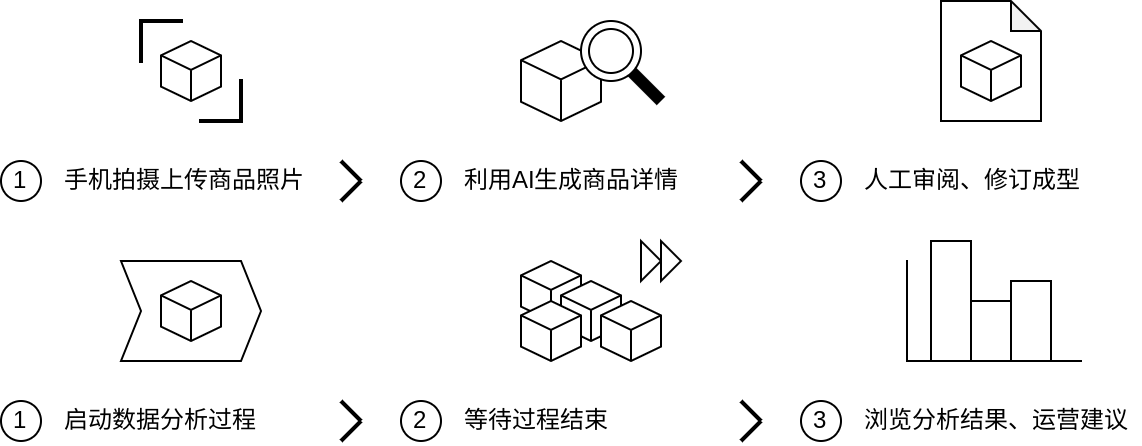
\includegraphics[width=0.8\textwidth]{./imgs/ai-owner-workflow.png}
	\caption{商家端AI功能总览}
	\label{fig:ai-owner-workflow}
\end{figure}

面向零售行业从业者的AI特性主要围绕着商品设计和图表分析展开。这两个业务板块实际上是以宣传为目的、以市场需要为导向的文本编纂;对营业中的各项数值在不同时间段中的变化趋势、不同周期的重复规律的研究。显然,不管是专业文本编纂还是销售数据挖掘都一定程度上超出了一般零售行业在店从业人员的能力范围。

对于一般的连锁店或其他类型的多店面实体零售企业,门店可以通过系统联网、数据同步的方式将这两项工作转移到企业本体的研发、市场部门,运用专业文学工作者、数据分析人员的专业能力来缓解这样的矛盾,一定程度上也有助于同品牌店面行为的标准化和品牌形象的塑造。

然而,这样的做法为每个特定的店面制定相应的经营策略的成本是较高的,并且将会对企业的相关资源造成较大的压力,但若是将每个店面的数据整合处理协同考虑,再分发统一的策略,又会使得各个店面效率的上限下降。并且,这样的运营模式一定程度上忽视了在店管理人员、其他工作人员对店面及其周边市场情况的了解,没有充分利用到不同类型、不同位置工作人员的具体能力素养。

对于自由程度较高的连锁店、加盟店或个体户,实际商品文案与广告的编写、商品备货策略的制定、市场趋势的预测和最终商业决策的施行一般均由该店面所对应管理者(如店长、店主等)进行。明显地,这对相关人员的文学素养、计算机等数字设备使用的熟练程度和“洞察力”(在特定情况下推理、判断并反映事物之间的因果关系的能力)提出了较高的要求。

该部分商家端AI功能,如图 \ref{fig:ai-owner-workflow} 所示,致力于缓解甚至根治这些问题。

\subsection{商品设计辅助}

\begin{figure}[htbp]
	\centering
	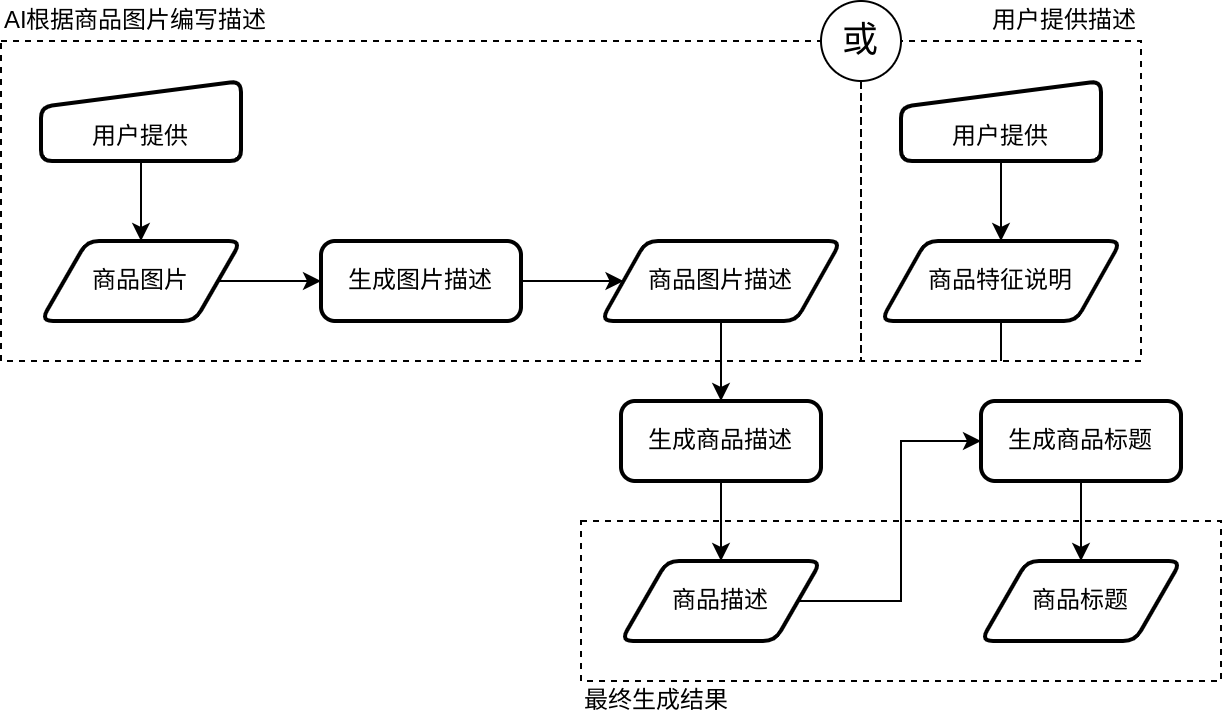
\includegraphics[width=0.8\textwidth]{./imgs/ai-writeup.png}
	\caption{AI商品设计辅助的执行流程图:其中上部两个的虚线框中内容所示不同输入和执行过程理论上可相互替换,本设计采用左侧部分的流程。}
	\label{fig:ai-writeup}
\end{figure}

为了缓解从业者在执行传统零售数字化的过程中遇到的难以编写高质量商品文案的问题,该设计包含一项特色AI功能:商品设计辅助。从业者提供商品对应的图片,也可以继续提供额外的参考资料,而后AI便可以根据这些信息产生对应的商品资料,从业者既可以根据实际情况直接采用生成结果,也可以在结果的基础上进行人工修改,较为具体的执行过程如图 \ref{fig:ai-writeup} 所示。

\subsubsection{编写文案}

与本设计的执行流程,利用AI编写出高质量的文案的条件可以归纳为以下几点:

\begin{itemize}
    \item LLM类型适合商业宣传性文案的编写
    \item LLM上下文窗口(context window)足够大
    \item LLM文字理解、逻辑推理、文学性能足够优越
    \item 使用的LLM具备多模态(multi-modal)特性或所使用的多个LLM中包含具有该特性的模型
    \item LLM具备足够高的节制度(moderation)
    \item 具备多模态特性的LLM图像细节(包括文本)的识别能力足够好
    \item 提示词(prompt)诱导LLM生成正确的、可自动处理的回复
    \item 提示词诱导LLM从图像提取更多信息
    \item 提示词最大程度上限制LLM在结果中包含臆想(hallucination)内容
\end{itemize}

对于文本生成的部分,笼统地说,任何适用于一般用途(也就是不是为某特定专业用途设计)的LLM都一定程度上具备编写商品文案的条件,只要合成合理的提示词或用于补全的文本就可以使用。本设计所对应的应用程序实现使用了阿里巴巴公司于“百炼”生成式AI服务平台提供的\verb|qwen-plus|商业大语言模型。若选用的LLM为进行对话(Instruct)进行过调优(如\verb|qwen-plus|),那么比较合理的输入是与“文案编写助手”的对话。本设计程序中生成商品描述提示词对话如下:

\begin{itemize}
    \item[] \textbf{系统:}你是一个处理商业资料的智能助手,不会输出问题答案以外的任何信息。
    \item[] \textbf{用户:}请根据以下提示编写可以吸引到潜在客户的网店产品介绍文案,400字以上,并且整理成适当长度的自然段。但是请尽可能不要对图片没有提及的商品情况和商店服务作出假设。以下是该产品图片的描述:\textit{(产品图片描述)}\dots
    \begin{itemize}
        \item[] \textbf{(提取图片文字时)}\dots 以下是从这个图片中发现的文字(若图片中没有文字,则可能会是无意义信息):\textit{(产品图片文字)}
        \item[] \textbf{(提供额外上下文时)}\dots 以下是店主附加的信息,请参考:\textit{(附加参考材料)}
    \end{itemize}
\end{itemize}

从图 \ref{fig:ai-writeup} 可见用于编写商品描述的材料可以来源于用户直接输入对目标商品的描述性文字,和交由额外模型处理的图片输入具有相似的效果。但是,采用这种输入方式的文案编写过程对营业者提出了新的要求,某种程度上相当于将对文学素养、宣传材料撰写能力的要求化为了对产品特征表达能力的要求,虽然同样是对“高门槛”问题的缓解,但不如输入图片的处理方式彻底\footnote{实际上,输入图片同样会对用户提出图像质量把控的要求。但明显地,一般用户满足该要求的概率相对而言是更高的,并且学会拍摄清晰照片的难度也更低。}。

如果使用性能较为强大的多模态模型(如开源的“千问”系列 \verb|Qwen2.5-VL| 模型),实际上可以将图片理解、描述的步骤和实际商品详情生成的步骤整合。在本设计的实现中考虑到大规模的多模态模型云服务对应的成本较高,并且输出速度一般慢于仅文本的大模型,故将两个步骤拆分,运用不同的模型处理。该设计中运用的视觉理解多模态大模型为“百炼”的商业大模型 \verb|qwen-vl-plus| ,程序中生成商品图片描述的提示词对话如下:

\begin{itemize}
    \item[] \textbf{系统:}你是一个处理商业资料的智能助手,不会输出问题答案以外的任何信息。
    \item[] \textbf{用户:}
    \begin{itemize}
        \item[] \textbf{(商品图片数据)}
        \item[] \textbf{(文字信息)} 该图片中包含一个商品,请用尽可能详细的语言描述该商品的外观特点,以便于后续无法查看该图片的其他模型处理。
    \end{itemize}
\end{itemize}

此外,程序中从商品图片中提取文字所使用的模型为“百炼”提供的商用特化模型 \verb|qwen-vl-ocr| ,提示词对话如下:

\begin{itemize}
    \item[] \textbf{系统:}你是一个处理商业资料的智能助手,不会输出问题答案以外的任何信息。
    \item[] \textbf{用户:}
    \begin{itemize}
        \item[] \textbf{(商品图片数据)}
        \item[] \textbf{(文字信息)} 该图片中包含一个商品,请发现该商品外观中包含的所有文字。但如果没有发现文字,也请如实回答。
    \end{itemize}
\end{itemize}

\subsubsection{建议定价}

对于一些特殊的零售细分行业、比较不常见的店面地段和无标准或习惯定价的商品种类,商品的最优定价并不明显。针对这一类较为特殊的情况,该设计提供一个参考定价生成功能,可以利用前文提及的商品描述和(可选的)附加参考材料来生成一个用于参考的商品价格。鉴于定价的过程逻辑性比较强,虽然该过程理论上可以采用一般大模型作为生成价格的算法,此处作为特殊情况采用了具备内省\footnote{即所谓“深度思考”(deep thinking)功能}(reflection)能力的大语言模型。这类模型中十分知名的是深度求索公司发布的开源模型“DeepSeek R1”,但为了缓解这类模型输出结果较为缓慢(模型较大并且具有思考过程)的问题,该设计采用(云上托管的)阿里巴巴发行的开源大模型“QwQ”。

显然,该过程需要输出的是价格的表示(于第 \ref{sec:foundation} 部分中提及的RmCore模块中的Price类型),但由于众所周知大语言模型的输出格式是较为随机的,此处采用许多常见文本模型具备的将输出规范为特定结构的JSON对象的功能。经过格式优化适合浏览的提示词对话如下:

\begin{itemize}
    \item[] \textbf{系统:}你是一个处理商业资料的智能助手,不会输出问题答案以外的任何信息。
    \item[] \textbf{用户:}请根据以下信息猜测该商品的价格。输出格式:
    \item[] \verb|{|
    \begin{itemize}
        \item[] \verb|"unit": 单位个或单位克|
        \item[] \verb|"price": 单位价格人民币分|
        \item[] \verb|"pricing": 计价方式|
    \end{itemize}
    \item[] \verb|}|
    \item[] 例如“可乐一罐卖3元”表示为
    \item[] \verb|{"unit": 1, "price": 300, "pricing": "Package"}|,
    \item[] “苹果一斤卖6元”表示为
    \item[] \verb|{"unit": 500, "price": 600, "pricing": "Weight"}|,
    \item[] 还请不要输出任何无关内容。以下是该产品图片的描述:\textit{(产品图片描述)}\dots
    \begin{itemize}
        \item[] \textbf{(提取图片文字时)}\dots 以下是从这个图片中发现的文字(若图片中没有文字,则可能会是无意义信息):\textit{(产品图片文字)}
        \item[] \textbf{(提供额外上下文时)}\dots 以下是店主附加的信息,请参考:\textit{(附加参考材料)}
    \end{itemize}
\end{itemize}

由于JSON格式的技术限制,\verb|pricing|枚举类型部分无法限制大模型的输出为合法值。桌面商家端应用程序此部分在后期反序列化进一步进行格式检查。

\subsubsection{提供额外参考}

前文提及用户可以在生成商品详情、标题和(可选地)价格时可以选择提供额外的资料给AI。因为在执行这些过程的时候,实际上大模型并不知悉门店的目标客群和运营情况、不清楚从业者的盈利目标,也不知道目前社会经济情况和特定商品的具体细节,但所有细节都将成为生成这下结果的重要参考。因此,这个特性是用户自主调优模型输出的重要的,也是较为易于理解的手段。

\subsection{营业数据分析}

为了缓解从业者在经营过程中需要分析销售数据,但是却不完全具备数据挖掘专家的专业能力的问题,该设计包含另一个特色AI功能:智能销售数据图表分析。分析界面软件将收集系统中与时间有关的各项数据指标,并通过图表展示其长时间的趋势、短时间的规律,而后利用AI解读图表蕴含的规律,提出合理的经营建议,而经营者可以通过参考AI给出的分析文字来轻松得知运营的规律和趋势情况,更可以以AI给出的建议为进一步规划营业计划的基础。

营业数据种类是多样的,分析的方式也同样种类丰富。为此,本设计中定义“营业数据”为零售商业运营的过程中与特定事件点(一般精确到秒或分钟)相关联的相互无直接关联的数值数据,比如顾客结算产生营运收入的事件对应的时间-数值(收入)元组,或者门店进货产生费用的时间-数值(支出)元组。通过以不同的时间间隔对这些数据进行整理、分类或累加,可以得出适合用于制图的数据。

\subsubsection{图表生成}

利用足够高的上下文长度,一定长度的原始数据可以以一般自然语言编码并被直接添加到模型的输入之中。然而这种处理方式在较少的数据(如一个月之间的收入)上就会占用大量的词法标记(lexical token),造成较为高昂的成本,因而这种处理方式在处理较多的原始数据的适合是并不实用的。并且这种处理方式并不能对用户给出较为直观的数据预览,仅适用于自动的分析方式。另一个向AI提供图表而不是原始数据的好处是将时间数列(time series)转化为二维平面上位置(折线图)、位置-强度(热力图)或其他统计学模型的表示,相当于将一部分繁重的统计任务从AI转移到了专用的表格数据、数值数据处理模块,理论上有助于AI对数据的深入分析。

为了使从业者能够直观的看到数据长期的趋势和短期的规律,也为了便于其后AI对数据进行进一步的分析,本设计的统计应用程序对任何输入到系统的时间序列数据,统一生成如下几种图表:

\begin{table}[htbp]
    \centering
    \begin{tabular}{|c|c|c|c|c|}
        \hline
        名称 & $x$轴 & $y$轴 & 强度 & 分析模式\\
        \hline
        周规律热力图 & 小时 & 星期 & 数值 & 观察后思考 \\
        \hline
        月规律热力图 & 小时 & 月份 & 数值 & 观察后思考 \\
        \hline
        周框图 & 星期 & 数值 & --- & 观察并思考 \\
        \hline
        月框图 & 月份 & 数值 & --- & 观察并思考 \\
        \hline
        日期折线图 & 日期 & 数值 & --- & 观察并思考 \\
        \hline
        周折线图 & 周数 & 数值 & --- & 观察并思考 \\
        \hline
    \end{tabular}
    \caption{提供用户浏览和AI推理分析的图表列表}
	\label{tab:graphs}
\end{table}

其中“周规律热力图”、“月规律热力图”可以形象地展示出对于数值每日的分布规律与一周中不同天或一年中不同月份的关系。用户(和AI)不但可以从中观察到数值在一天内的变化规律,还可以观察到这个规律本身根据不同条件发生的变化。借此可以推测用户的购买习惯和零售门店的营业情况,并据此制定营业策略。两个框图分别展示按星期和月份整理的对应数值的分布情况。在框图上可以直观地看到数值的$\frac{1}{4}$、$\frac{3}{4}$分位值、中位数等关键统计值。据此可以较为容易地比较不同星期或月份数值的分布规律的区别。最后的两个折线图则是按照(用户)选择的时间段分别按天或按周整理的数字变化折线图。

\subsubsection{图表理解}

本设计图表理解部分针对不同的图表类型采用两种复杂程度不同的分析流程:

\begin{itemize}
    \item \textbf{先观察再分析(stare then ponder):}先利用多模态大模型进行图表关键内容、规律的提取,再将提取结果输入到适于处理文本、逻辑推理的大语言模型来分析因果关系和生成营业策略建议。
    \item \textbf{边观察边分析(stare and ponder):}
\end{itemize}

\subsubsection{营业策略建议}

\subsection{库存审计}